\documentclass{article}
\usepackage[utf8]{inputenc}
\usepackage{hyperref}
\usepackage{amsmath}
\usepackage{amsfonts}
\usepackage{graphicx}
\usepackage{enumitem}
\usepackage{wrapfig}
\graphicspath{ {./images} }


\title{IPhO Class - Oscillations \& Waves}
\author{
    Tan Chien Hao\\
    \texttt{www.tchlabs.net}\\
    \texttt{Telegram @tch1001}
    % new collaborators add your name and contact here!
}

\date{\today}
\begin{document}
\newif\ifpaper

% TOGGLE ANSWER HERE
\paperfalse 

\maketitle
\tableofcontents
\section{Phasors Trick}
\section{Lagrangian Mechanics for Oscillations}
\subsection{Coupled Cart and Pendulum}
A pendulum of mass $\mathrm{m}$ and length $\ell$ is hung from a support of mass $M$ which is free to move horizontally on a frictionless rail. Find the equations of motion. For small oscillations, find the normal modes and their frequencies. \\
\begin{figure}[h]
    \centering
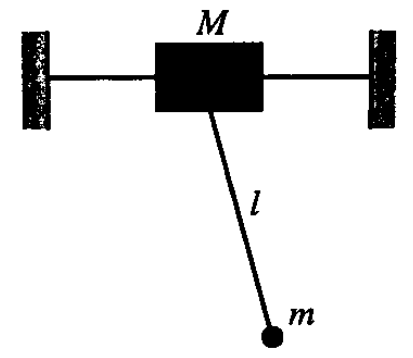
\includegraphics[width=0.4\linewidth]{images/cartpendulum.png}
\end{figure}\\
Ans: 
\begin{align}
&(M+m) \ddot{x}+m \ell\left(\ddot{\theta} \cos \theta-\dot{\theta}^2 \sin \theta\right)=0 \\
&\ell \ddot{\theta}+\ddot{x} \cos \theta=-g \sin \theta \\
&\omega=0, \ \theta=0,\ x= A t \\ 
&\omega=\sqrt{1+\frac{m}{M}} \sqrt{\frac{g}{\ell}}, \ x=-\frac{m \ell}{M+m} \theta
\end{align}

\subsection{Coupled Sliding Cart and Pendulum}
A mass $M$ slides down a frictionless plane inclined at angle $\beta$. A pendulum, with length $\ell$ and mass $m$, is attached to $M$. Find the equations of motion, and also the normal modes of small oscillations. \\
\begin{figure}[h]
    \centering
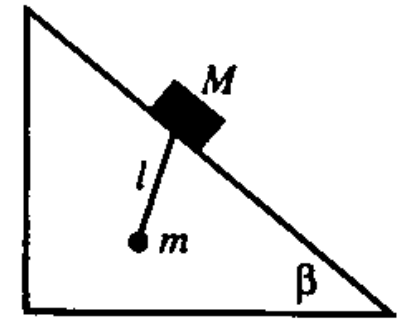
\includegraphics[width=0.4\linewidth]{images/slidingcartpendulum.png}
\end{figure}\\
Ans: 
\begin{align}
& (M+m) \ddot{z}+m \ell\left(\ddot{\theta} \cos (\theta+\beta)-\dot{\theta}^2 \sin (\theta+\beta)\right)=(M+m) g \sin \beta \\ 
& \ell \ddot{\theta}+\ddot{z} \cos (\theta+\beta)=-g \sin \theta \\ 
& \omega=0 \\
& \omega=\sqrt{1+\frac{m}{M}} \sqrt{\frac{g \cos \beta}{\ell}} 
\end{align}
\subsection{Coupled Rod and Bead}
A mass $M$ is fixed at the right-angled vertex where a massless rod of length $\ell$ is connected to a very long massless rod. A mass $m$ is free to move frictionlessly along the long rod. The rod of length $\ell$ is hinged at a support, and the whole system is free to rotate, in the plane of the rods, about the support. Let $\theta$ be the angle of rotation of the system, and let $x$ be the distance between $m$ and $M$. Find the equations of motion. Find the normal modes when $\theta$ and $x$ are both very small. Note that the range of validity of one mode is limited as the values will soon fall outside the validity of our small-variable approximations.
\begin{figure}[h]
    \centering
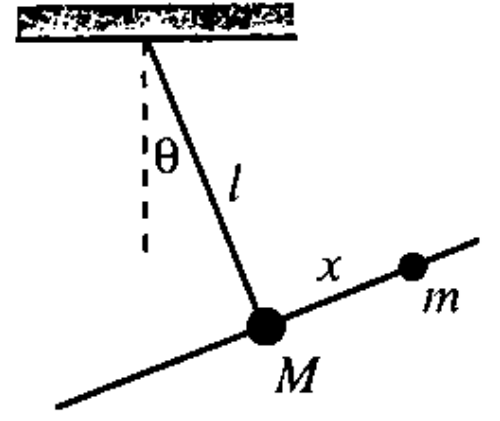
\includegraphics[width=0.4\linewidth]{images/rodandbead.png}
\end{figure}\\
Ans: 
\begin{align}
& \ell \ddot{\theta}+\ddot{x}=x \dot{\theta}^2-g \sin \theta\\
& M \ell^2 \ddot{\theta}+m \ell(\ell \ddot{\theta}+\ddot{x})+m x^2 \ddot{\theta}+2 m x \dot{x} \dot{\theta}=-M g \ell \sin \theta- m g \ell \sin \theta-m g x \cos \theta \notag \\
& x(t)=0, \quad \omega=\sqrt{\frac{g}{\ell}} \\ 
& x(t)=A \cosh \left(\sqrt{\frac{m g}{M \ell}} t+\phi\right), \quad \theta= B \cosh \left(\sqrt{\frac{m g}{M \ell}} t+\phi\right)
\end{align}
\end{document}